% !TeX encoding = UTF-8
% !TeX spellcheck = russian-aot
% !TeX program = xelatex
\documentclass[14pt, a4paper, titlepage]{extarticle}

\usepackage[english, main=russian]{babel}
\usepackage{fontspec}
\setmainfont{Times New Roman}
\usepackage[left=30mm, right=15mm, top=20mm, bottom=20mm]{geometry}

\usepackage{microtype}
\usepackage{lettrine}
\renewcommand{\LettrineTextFont}{\upshape}
\usepackage{graphicx}
\usepackage{float}

\usepackage{pgfplots} % Графики
\pgfplotsset{width=.8\textwidth, compat=1.9}

\usepackage{authblk}

\usepackage{csquotes}
\usepackage[left={<<}, right={>>}, leftsub={„}, rightsub={“}]{dirtytalk}
\usepackage[backend=bibtex]{biblatex}
\addbibresource{source.bib}

\linespread{1.3}
\righthyphenmin=2
\parskip=0pt
\parindent=1.25cm

\title{Моделирование систем. Практика 6. Вариант 1}
\author{Р.\,Абдуллин, В.\,Верхотуров \\  БСБО-05-20}
\affil{РТУ МИРЭА}

\usepackage{hyperref}
\hypersetup{pdftitle={Моделирование систем. Практика 6}, pdfauthor={Р. Абдуллин, В. Верхотуров}}

\begin{document}
	\maketitle
	
	\section{Модель}
	
	\begin{figure}[H]
		\centering
		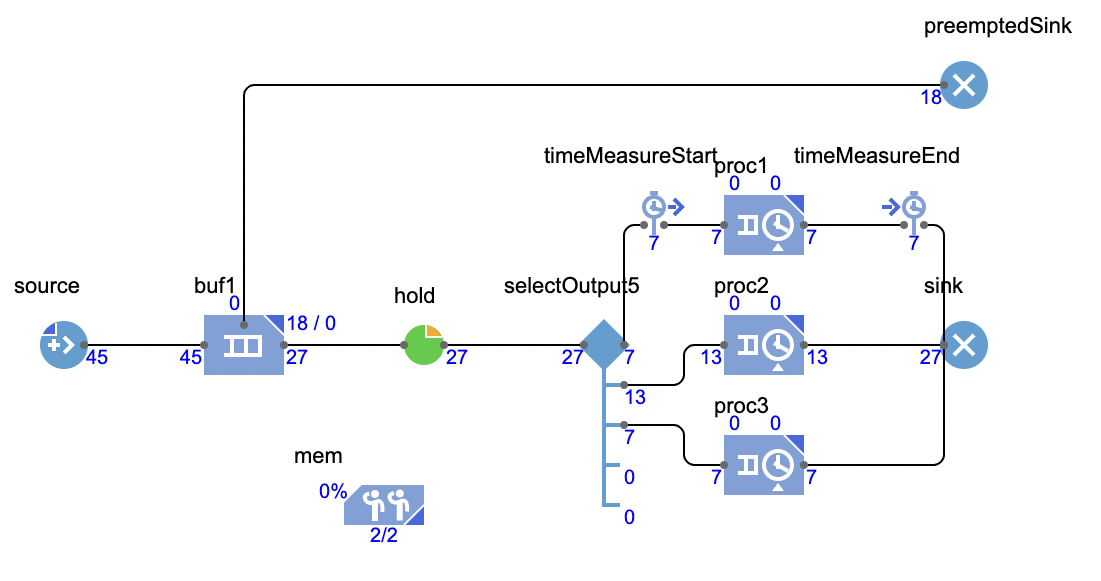
\includegraphics[width=.9\textwidth]{model}
		\caption{Параллельная вычислительная система с использование общих ресурсов}
	\end{figure}

	\begin{figure}[H]
		\centering
		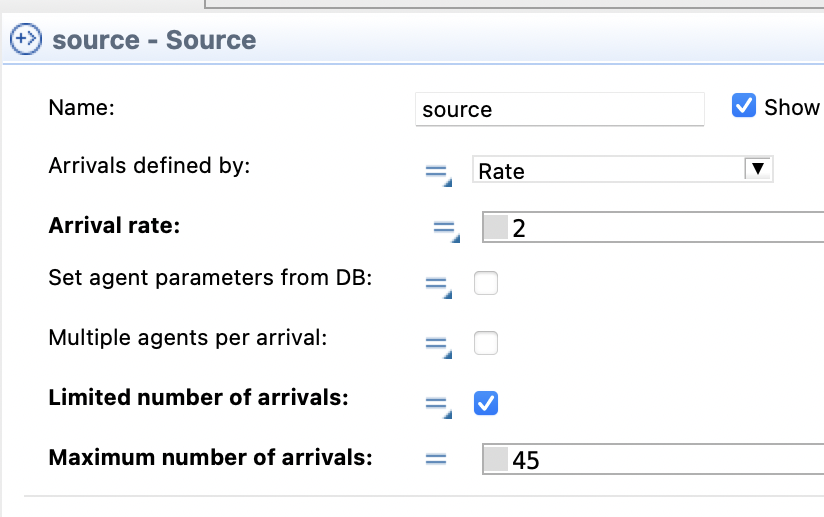
\includegraphics[width=.9\textwidth]{source}
		\caption{Source}
	\end{figure}

	\begin{figure}[H]
		\centering
		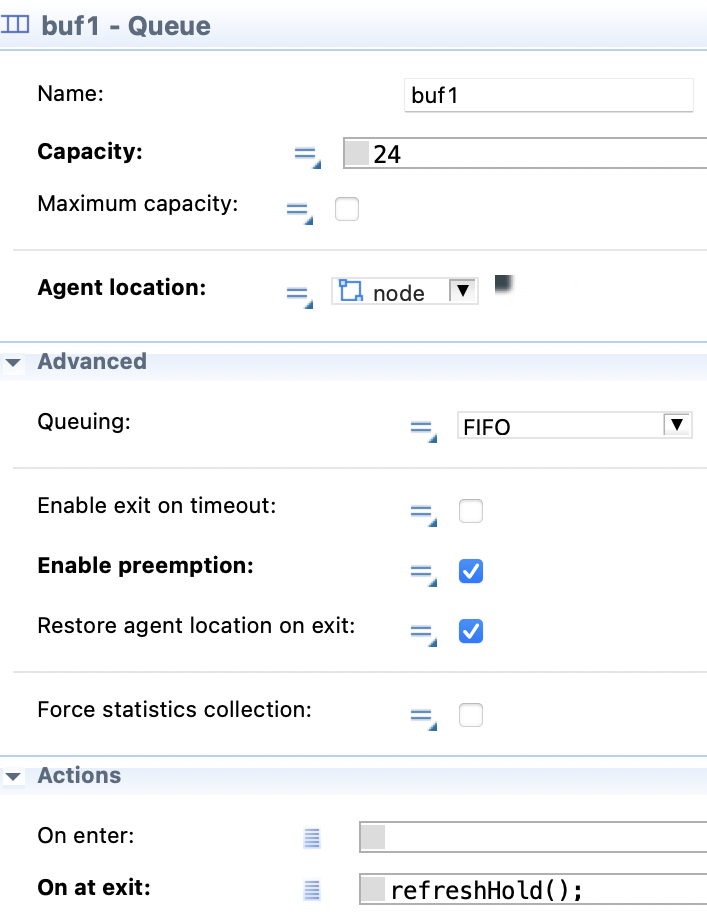
\includegraphics[width=.9\textwidth]{buf1}
		\caption{Buf1}
	\end{figure}

	\begin{figure}[H]
		\centering
		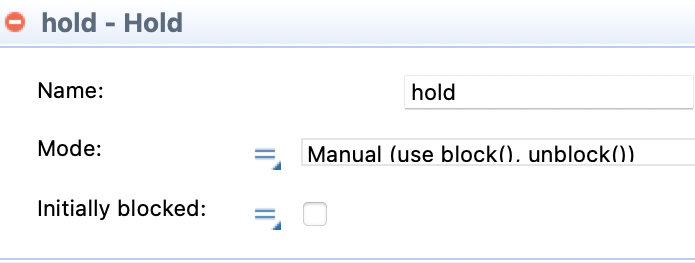
\includegraphics[width=.9\textwidth]{hold}
		\caption{Hold}
	\end{figure}

	\begin{figure}[H]
		\centering
		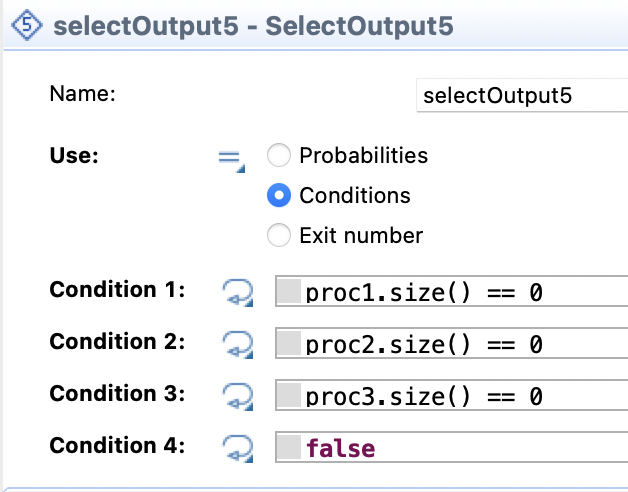
\includegraphics[width=.9\textwidth]{selectOutput5}
		\caption{selectOutput5}
	\end{figure}

	\begin{figure}[H]
		\centering
		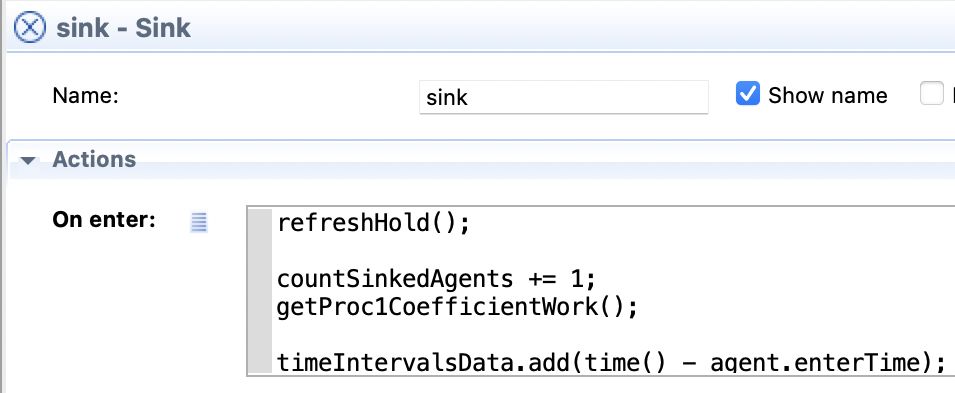
\includegraphics[width=.9\textwidth]{sink}
		\caption{Sink}
	\end{figure}

	\begin{figure}[H]
		\centering
		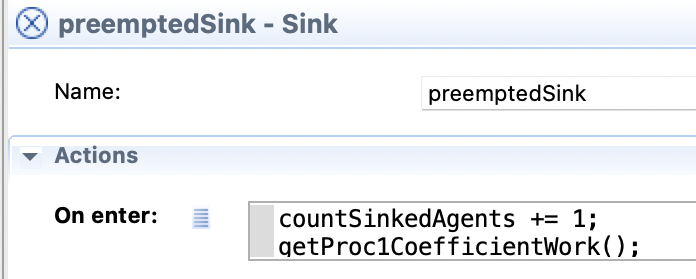
\includegraphics[width=.9\textwidth]{preemptedSink}
		\caption{PreemptedSink}
	\end{figure}

	\begin{figure}[H]
		\centering
		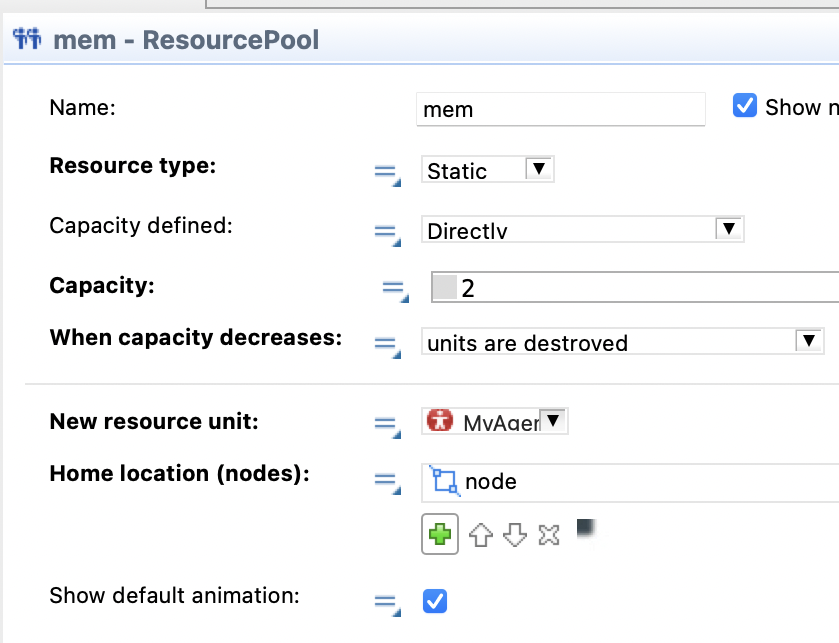
\includegraphics[width=.9\textwidth]{mem}
		\caption{Memory}
	\end{figure}
	
	\begin{figure}[H]
		\centering
		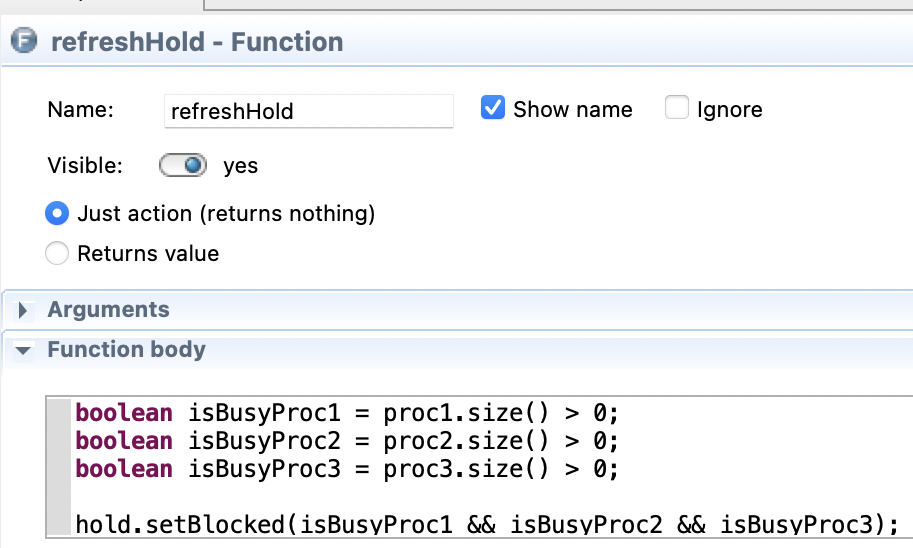
\includegraphics[width=.9\textwidth]{refreshHold}
		\caption{RefreshHold}
	\end{figure}

	\begin{figure}[H]
		\centering
		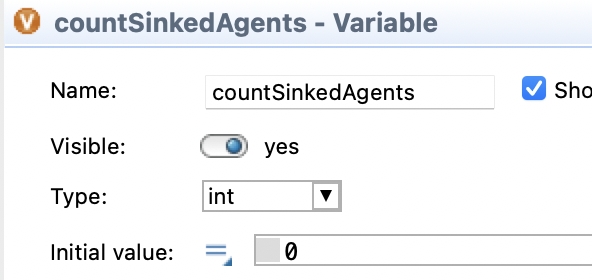
\includegraphics[width=.9\textwidth]{countSinkedAgents}
		\caption{CountSinkedAgents}
	\end{figure}

	\begin{figure}[H]
		\centering
		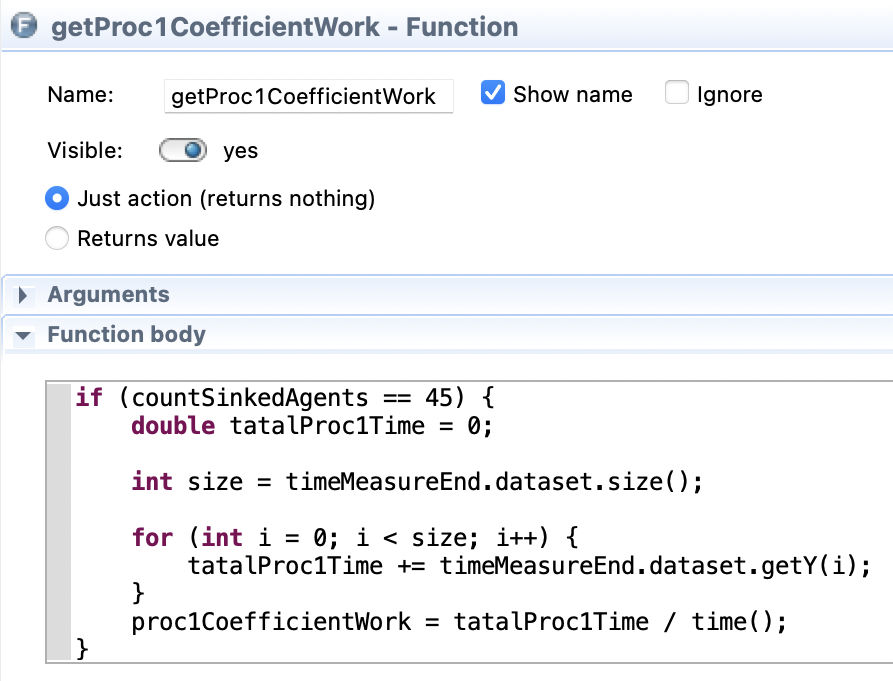
\includegraphics[width=.9\textwidth]{getProc1CoefficientWork}
		\caption{GetProc1CoefficientWork}
	\end{figure}

	\begin{figure}[H]
		\centering
		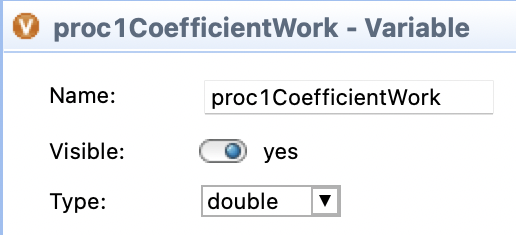
\includegraphics[width=.9\textwidth]{proc1CoefficientWork}
		\caption{proc1CoefficientWork}
	\end{figure}
	
	\section{Описание модели}
	
	\begin{description}
		\item[Правило прибытия (сек.)] Интенсивность, 2;
		\item[Максимальное кол-во сообщений] 45;
		\item[Размер буфера] 24;
		\item[] Время обработки:
		\begin{description}
			\item[процессора \textnumero~1] 28;
			\item[процессора \textnumero~2] 25;
			\item[процессора \textnumero~3] 28;
			
		\end{description}
		\item[Контролируемый параметр] резидентное время, коэффициент загрузки процессора (использовать timeMeasureStart и timeMeasureEnd);
		\item[Блок] процессор 1.
	\end{description}
	
	
	\section{Резидентное время}
	
	\begin{figure}[H]
		\centering
		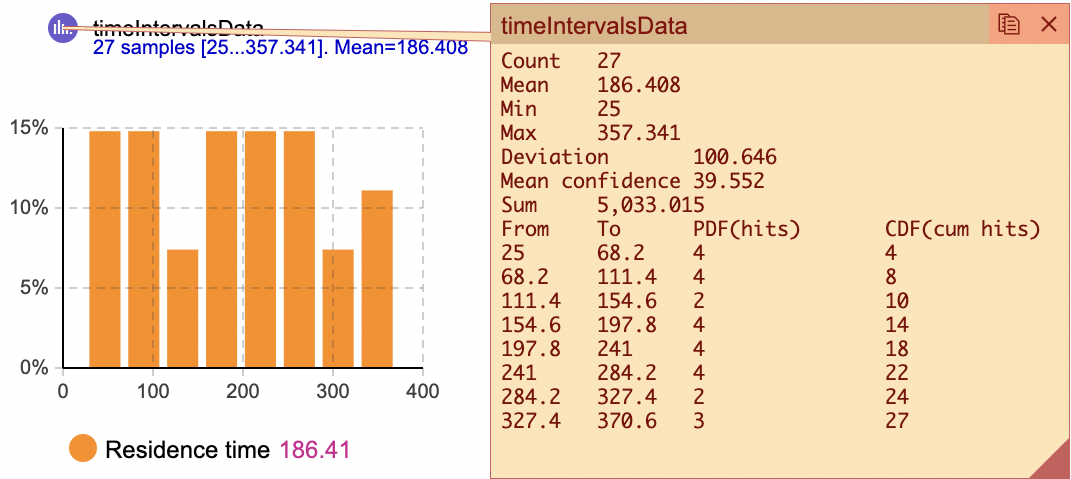
\includegraphics[width=.9\textwidth]{residenttime}
		\caption{Коэффициент загрузки процессора}
	\end{figure}
	
	\section{Резидентное время}
	
	\begin{figure}[H]
		\centering
		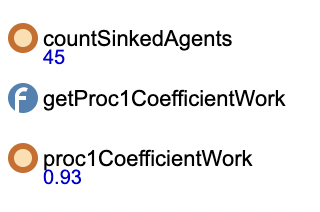
\includegraphics[width=.3\textwidth]{coef}
		\caption{Коэффициент загрузки процессора}
	\end{figure}
	
	\section{Визуализация}
	
	\begin{figure}[H]
		\centering
		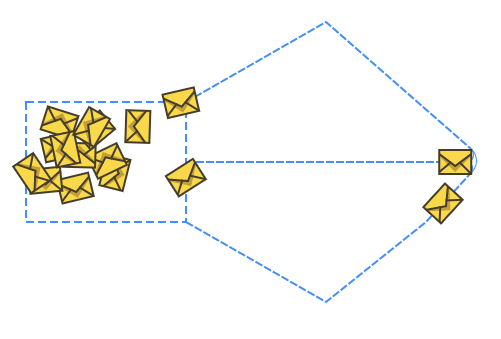
\includegraphics[width=.5\textwidth]{visualisation}
		\caption{Визуализация модели}
	\end{figure}
	
	
	

	
	\section{Анализ системы}
	
	18 сообщений из 45 были утеряны в буфере. При памяти, вместительностью 2, невозможна работа одновременно трех процессоров.
	
	\section{Вывод}
	
	Для улучшения модели можно увеличить очередь, объем разделяемой памяти.
	
	
\end{document}